\section{Polar Observers, Extremal Kerr and NHEK Structure}
\label{sec:extremal_nhek_and_polar}

\subsection{Extremal Kerr Black Holes and the Critical Inclination}
\label{subsec:extremal_kerr_critical}
In the extreme Kerr limit ($|a| = M$), the outer event horizon and inner Cauchy horizon coalesce at coordinate radius $r_+ = r_- = M$. The metric horizon function $\Delta(r) = (r - M)^2$ develops a double root, and the exterior spherical photon orbit parameters \eqref{eq:spherical_xi}--\eqref{eq:spherical_eta} simplify to:
\begin{align}
    \xi_{\rm ext}(r) &= M + 2r - \frac{r^2}{M}, \label{eq:extremal_xi} \\
    \eta_{\rm ext}(r) &= \frac{r^3\left[4M^3 - r(r - 3M)^2\right]}{M^2(r - M)^2}. \label{eq:extremal_eta}
\end{align}
As the generating spherical orbit approaches the horizon from the exterior ($r \to M^+$), these parameters approach finite, non-zero limiting values:
\begin{equation}
    \lim_{r \to M^+} \xi_{\rm ext}(r) = 2M, \qquad \lim_{r \to M^+} \eta_{\rm ext}(r) = 3M^2.
    \label{eq:extremal_horizon_limits}
\end{equation}

Evaluating the Carter vertical radicand function $B(r; \theta_o)$ defined in \eqref{eq:carter_B_u} directly at the horizon $r = M$ yields:
\begin{equation}
    B(M; \theta_o) = 3M^2 + M^2\cos^2\theta_o - 4M^2\cot^2\theta_o = M^2 \left( 3 - C(\theta_o) \right),
    \label{eq:B_horizon_extremal}
\end{equation}
where the inclination function $C(\theta_o)$ is:
\begin{equation}
    C(\theta_o) \equiv \frac{\cos^2\theta_o \left(3 + \cos^2\theta_o\right)}{\sin^2\theta_o} \ge 0.
    \label{eq:def_C_theta}
\end{equation}
The physical existence of real shadow boundary points requires $B(M; \theta_o) \ge 0$, which is satisfied if and only if $C(\theta_o) \le 3$. Setting $C(\theta_{\rm crit}) = 3$ yields a quadratic equation in $\cos^2\theta_{\rm crit}$:
\begin{equation}
    \cos^4\theta_{\rm crit} + 6\cos^2\theta_{\rm crit} - 3 = 0 \implies \cos^2\theta_{\rm crit} = 2\sqrt{3} - 3 \approx 0.4641016,
    \label{eq:theta_crit_derivation}
\end{equation}
defining the critical observer inclination $\theta_{\rm crit}$ \cite{Bardeen1973,Gralla2020}:
\begin{equation}
    \theta_{\rm crit} = \arccos\left(\sqrt{2\sqrt{3} - 3}\right) \approx 47.058597^\circ \approx 0.821323 \text{ rad}.
    \label{eq:theta_crit_val}
\end{equation}

\subsection{Near-Horizon Extreme Kerr (NHEK) Vertical Segment}
\label{subsec:nhek_vertical_segment}
The critical angle $\theta_{\rm crit}$ partitions the observational phenomenology of extremal Kerr black holes into two distinct geometric regimes:
\begin{enumerate}
    \item \textbf{Subcritical Observers ($\theta_o < \theta_{\rm crit}$):}  
    For inclinations closer to the pole than $\theta_{\rm crit}$, $C(\theta_o) > 3$, implying $B(M; \theta_o) < 0$. The turning points $B(r; \theta_o) = 0$ occur strictly exterior to the horizon ($r_{\min} > M$). The shadow boundary is closed, strictly convex, and smooth, with the event horizon completely shielded from direct celestial view by the photon capture barrier.
    
    \item \textbf{Supercritical Observers ($\theta_o > \theta_{\rm crit}$, e.g., Equatorial $\theta_o = 90^\circ$):}  
    For inclinations closer to the equator than $\theta_{\rm crit}$, $C(\theta_o) < 3$, so $B(M; \theta_o) > 0$. The exterior curved boundary reaches the horizon at $r = M$, terminating at horizontal impact coordinate:
    \begin{equation}
        \alpha_{\rm pro} = -\frac{\xi_{\rm ext}(M)}{\sin\theta_o} = -\frac{2M}{\sin\theta_o},
    \end{equation}
    with non-zero vertical coordinate $\pm \beta_{\max}$, where:
    \begin{equation}
        \beta_{\max} \equiv M \sqrt{3 - C(\theta_o)}.
        \label{eq:beta_max_nhek}
    \end{equation}
\end{enumerate}

To complete the closed boundary of the shadow, the termination points $(\alpha_{\rm pro}, \pm\beta_{\max})$ are joined by an exact vertical line segment:
\begin{equation}
    \alpha_{\rm NHEK} = -\frac{2M}{\sin\theta_o}, \qquad \beta \in [-\beta_{\max}, +\beta_{\max}].
    \label{eq:nhek_line_segment}
\end{equation}
Physically, this straight segment represents the projection of an infinite family of bound spherical photon orbits that reside on the infinitely extended throat of the Near-Horizon Extreme Kerr (NHEK) geometry \cite{BardeenPressTeukolsky1972,Gralla2020}. In the extremal limit, the coordinate distance to the horizon collapses, but the physical proper distance blows up, opening an infinite throat endowed with an enhanced $SL(2, \mathbb{R}) \times U(1)$ conformal isometry group. Photons with $\xi = 2M$ and Carter constants $\eta \in [4M^2\cot^2\theta_o - M^2\cos^2\theta_o, 3M^2]$ reside on radially unstable spherical photon orbits (separatrices) within this throat (with $\eta = 3M^2$ forming the marginally degenerate endpoint where $R''(M) = 0$), casting an exact vertical line on the observer's screen.

For an equatorial observer ($\theta_o = 90^\circ$), $C(\pi/2) = 0$, giving:
\begin{equation}
    \alpha_{\rm NHEK} = -2M, \qquad \beta \in [-\sqrt{3}M, +\sqrt{3}M],
    \label{eq:nhek_equatorial}
\end{equation}
forming the characteristic flat D-shaped vertical edge shown in \Cref{fig:kerr_shadow_extremal}.

\begin{figure}[!htbp]
    \centering
    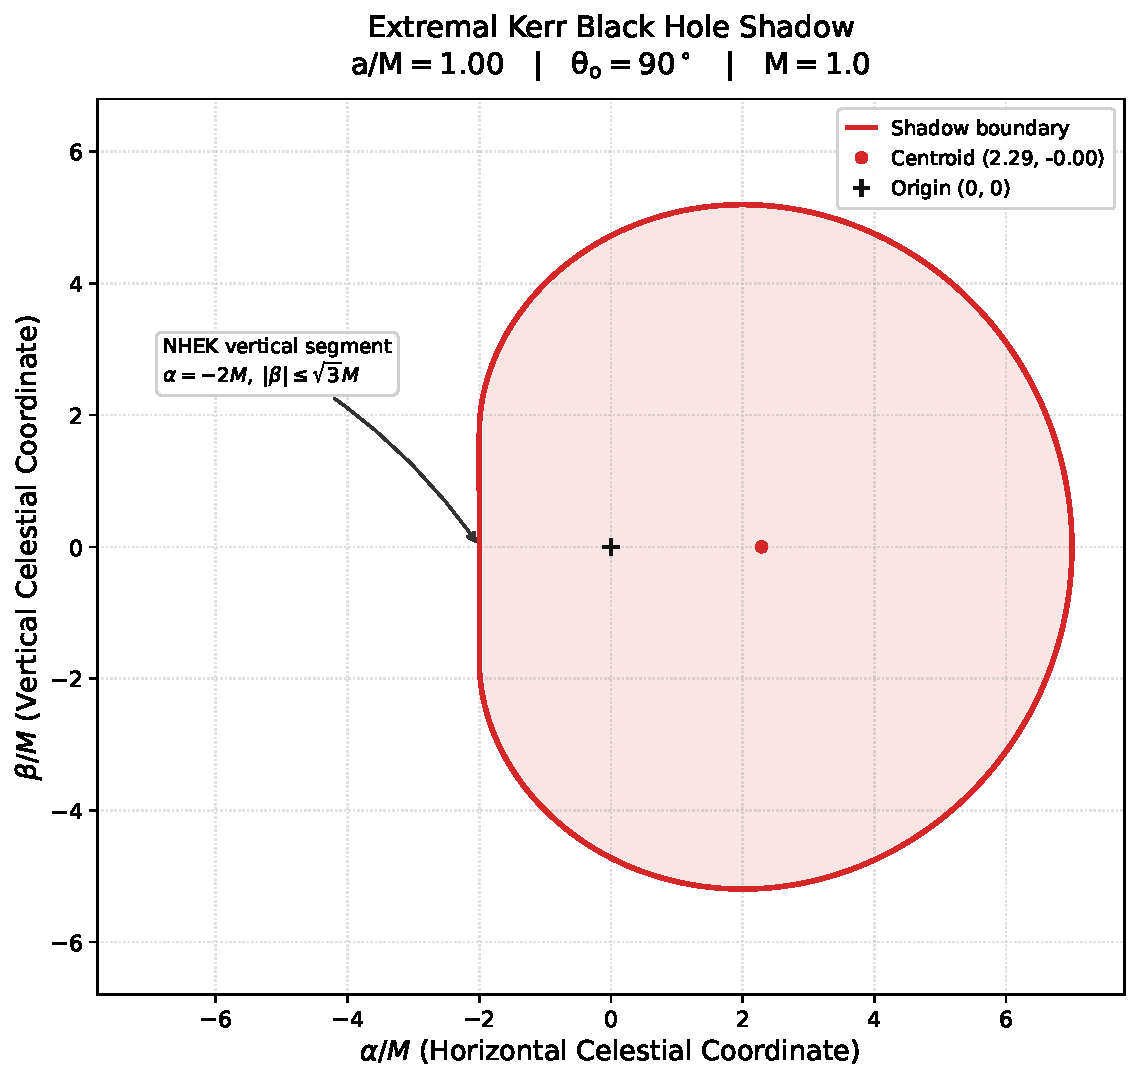
\includegraphics[width=0.58\textwidth]{kerr_shadow_extremal.pdf}
    \caption{Extremal Kerr black hole shadow ($M = 1.0, a = 1.0M, \theta_o = 90^\circ$). The prograde boundary is terminated by the vertical Near-Horizon Extreme Kerr (NHEK) line segment at $\alpha = -2M$, spanning $\beta \in [-\sqrt{3}M, +\sqrt{3}M]$ ($\beta_{\max} \approx 1.732M$), joining the smooth exterior curved branch at sharp $C^0$ corners.}
    \label{fig:kerr_shadow_extremal}
\end{figure}

\subsection{Multi-Inclination Comparison for Rapidly Rotating Black Holes}
\label{subsec:inclination_comparison}
The appearance of a black-hole shadow depends sensitively on the observer's line-of-sight inclination $\theta_o$. \Cref{fig:kerr_shadow_inclination_comparison} presents the verified shadow profiles for a rapidly rotating Kerr black hole ($a = 0.90M, M = 1.0$) across three representative observer inclinations:
\begin{equation}
    \theta_o \in \{15^\circ, 45^\circ, 90^\circ\}.
\end{equation}

\begin{figure}[!htbp]
    \centering
    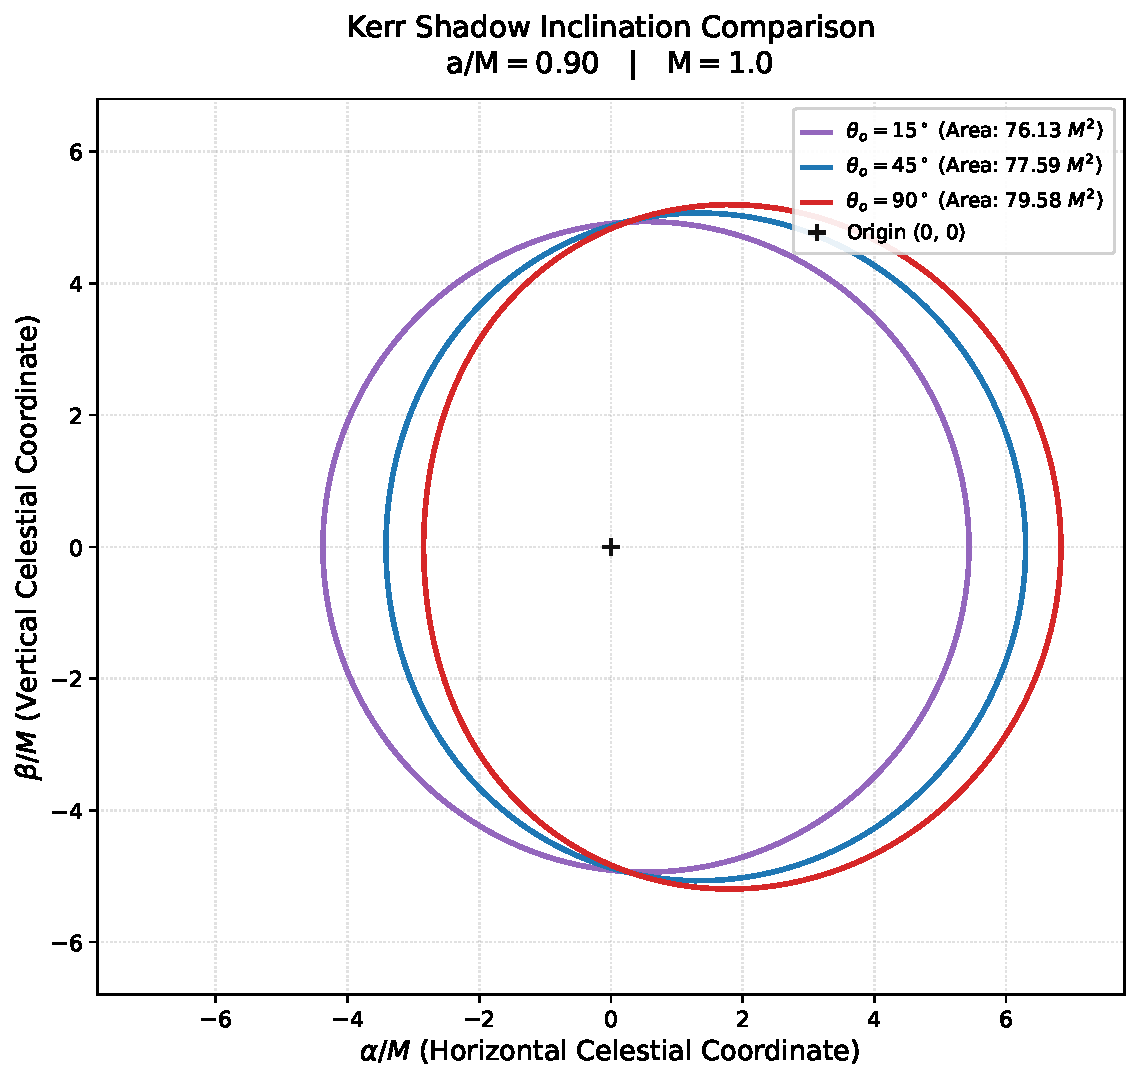
\includegraphics[width=0.58\textwidth]{kerr_shadow_inclination_comparison.pdf}
    \caption{Comparison of Kerr black hole shadow boundaries at $a/M = 0.90$ across observer inclinations $\theta_o = 15^\circ$ ($A = 76.13M^2$), $\theta_o = 45^\circ$ ($A = 77.59M^2$), and $\theta_o = 90^\circ$ ($A = 79.58M^2$). The profile transitions smoothly from an asymmetric, flattened D-shape at high inclination to a nearly circular silhouette near the pole.}
    \label{fig:kerr_shadow_inclination_comparison}
\end{figure}

The physical progression across inclinations exhibits clear geometric systematics:
\begin{itemize}
    \item \textbf{Equatorial Observer ($\theta_o = 90^\circ$):} The line of sight lies directly in the black hole's equatorial plane. Frame-dragging is maximally projected onto the celestial screen ($\sin\theta_o = 1$). Prograde photons can orbit as close as $r_{\rm ph}^+ \approx 1.56M$, compressing the prograde edge to $\alpha_{\min} \approx -2.84M$, whereas retrograde photons are held out at $r_{\rm ph}^- \approx 3.91M$, extending the retrograde edge to $\alpha_{\max} \approx +6.83M$. This creates maximal horizontal asymmetry ($D_{\mathrm{H}} = 9.68M, D_{\mathrm{V}} = 10.39M$), with the area centroid displaced to $\bar{\alpha} = +1.93M$.
    \item \textbf{Intermediate Observer ($\theta_o = 45^\circ$):} Because the projected spin vector is inclined by $45^\circ$, the asymmetric displacement of the centroid decreases to $\bar{\alpha} = +1.41M$, and the enclosed area contracts to $A = 77.59M^2$.
    \item \textbf{Near-Polar Observer ($\theta_o = 15^\circ$):} As the observer approaches the rotation axis, the apparent velocity of spacetime rotation projected perpendicular to the line of sight diminishes proportionally to $\sin\theta_o$. The centroid shift drops to $\bar{\alpha} = +0.53M$, and the horizontal and vertical diameters become nearly equal ($D_{\mathrm{H}} = 9.81M, D_{\mathrm{V}} = 9.88M$), yielding a nearly circular silhouette ($A = 76.13M^2$).
\end{itemize}

\subsection{Exact-Polar Observer Shadows ($\theta_o = 0^\circ$)}
\label{subsec:exact_polar_shadows}
For an observer situated precisely on the polar rotation axis ($\theta_o = 0^\circ$), axial symmetry requires that the black-hole shadow must be an exact circle centered at the origin of the celestial screen ($\alpha^2 + \beta^2 = R_{\rm pole}^2$).

In the polar limit $\theta_o \to 0$, $\cot^2\theta_o \to \infty$. To prevent the vertical radicand $\beta^2 = \eta + a^2\cos^2\theta_o - \xi^2\cot^2\theta_o$ from diverging to $-\infty$, the axial angular momentum of the generating spherical photon orbit must vanish identically:
\begin{equation}
    \xi(r_p) = 0 \iff M(r_p^2 - a^2) - r_p\Delta(r_p) = 0 \iff r_p^2(3M - r_p) - a^2(r_p + M) = 0.
    \label{eq:polar_orbit_equation}
\end{equation}
For any spin $a \in [0, M]$, \eqref{eq:polar_orbit_equation} has a unique physical root $r_p$ in the exterior interval $(M, 3M]$:
\begin{equation}
    r_p \in [1 + \sqrt{2}, 3]M.
    \label{eq:rp_range}
\end{equation}
At this polar radius, the Carter constant $\eta_p \equiv \eta(r_p)$ is strictly positive. Evaluating the screen radius in the limit $\theta_o \to 0$ gives:
\begin{equation}
    R_{\rm pole}(a) \equiv \sqrt{\eta(r_p) + a^2}.
    \label{eq:polar_circle_radius}
\end{equation}

\subsubsection{Derivation of the Polar Extremal Shadow Radius}
For an extremal black hole ($a = M$), \eqref{eq:polar_orbit_equation} becomes:
\begin{equation}
    r_p^2(3M - r_p) - M^2(r_p + M) = 0 \iff r_p^3 - 3M r_p^2 + M^2 r_p + M^3 = 0.
    \label{eq:extremal_polar_poly}
\end{equation}
Factoring out the root at $r = M$ gives:
\begin{equation}
    (r_p - M)\left( r_p^2 - 2M r_p - M^2 \right) = 0 \iff (r_p - M)\left[ (r_p - M)^2 - 2M^2 \right] = 0.
\end{equation}
The unique root exterior to the horizon ($r_p > M$) is:
\begin{equation}
    r_p = (1 + \sqrt{2})M \approx 2.41421356M.
    \label{eq:rp_extremal_val}
\end{equation}

To evaluate the Carter constant $\eta(r_p)$ at this radius, we introduce the dimensionless radial coordinate $x \equiv r/M$, so that the extremal Carter constant \eqref{eq:extremal_eta} takes the form:
\begin{equation}
    \frac{\eta_{\rm ext}(r)}{M^2} = \frac{x^3\left[ 4 - x(x - 3)^2 \right]}{(x - 1)^2}.
    \label{eq:extremal_eta_dimensionless}
\end{equation}
At the polar photon orbit, $x_p \equiv r_p/M = 1 + \sqrt{2}$. We evaluate each component systematically:
\begin{align}
    (x_p - 1)^2 &= \left(\sqrt{2}\right)^2 = 2, \label{eq:eval_denom} \\
    x_p^3 &= (1 + \sqrt{2})^3 = 1 + 3\sqrt{2} + 6 + 2\sqrt{2} = 7 + 5\sqrt{2}, \label{eq:eval_cube} \\
    x_p - 3 &= \sqrt{2} - 2 \implies (x_p - 3)^2 = 2 - 4\sqrt{2} + 4 = 6 - 4\sqrt{2}, \label{eq:eval_sq} \\
    x_p(x_p - 3)^2 &= (1 + \sqrt{2})(6 - 4\sqrt{2}) = 6 - 4\sqrt{2} + 6\sqrt{2} - 8 = -2 + 2\sqrt{2}, \label{eq:eval_prod} \\
    4 - x_p(x_p - 3)^2 &= 4 - (-2 + 2\sqrt{2}) = 6 - 2\sqrt{2}. \label{eq:eval_bracket}
\end{align}
Multiplying the cubic prefactor \eqref{eq:eval_cube} by the bracket \eqref{eq:eval_bracket} gives the numerator:
\begin{equation}
    x_p^3\left[ 4 - x_p(x_p - 3)^2 \right] = (7 + 5\sqrt{2})(6 - 2\sqrt{2}) = 42 - 14\sqrt{2} + 30\sqrt{2} - 20 = 22 + 16\sqrt{2}.
\end{equation}
Dividing by the denominator $(x_p - 1)^2 = 2$ from \eqref{eq:eval_denom} yields the exact Carter constant:
\begin{equation}
    \eta_{\rm ext}(r_p) = \frac{22 + 16\sqrt{2}}{2} M^2 = (11 + 8\sqrt{2}) M^2.
    \label{eq:eta_extremal_polar}
\end{equation}

The polar shadow screen radius is therefore:
\begin{align}
    R_{\rm pole}^2 &= \eta_{\rm ext}(r_p) + a^2 = (11 + 8\sqrt{2})M^2 + M^2 = (12 + 8\sqrt{2})M^2 \nonumber \\
    &= 4\left(3 + 2\sqrt{2}\right)M^2 = 4\left(1 + \sqrt{2}\right)^2 M^2.
    \label{eq:R_pole_squared_derivation}
\end{align}
Taking the positive square root yields the exact analytical result:
\begin{equation}
    R_{\rm pole}(M) = 2\left(1 + \sqrt{2}\right)M = \sqrt{12 + 8\sqrt{2}}M \approx 4.82842712M.
    \label{eq:R_pole_extremal_exact}
\end{equation}
Notice that $R_{\rm pole}(M) = 2 r_p$. The corresponding diameters and celestial area are:
\begin{align}
    D_{\mathrm{H}} &= D_{\mathrm{V}} = 2 R_{\rm pole} = 4\left(1 + \sqrt{2}\right)M \approx 9.656854M, \label{eq:extremal_polar_diameters} \\
    A &= \pi R_{\rm pole}^2 = 4\left(3 + 2\sqrt{2}\right)\pi M^2 \approx 73.2415M^2, \label{eq:extremal_polar_area}
\end{align}
matching the underlying high-resolution numerical observables to eight significant digits, consistent with the displayed values in \Cref{tab:shadow_observables}.

In the Schwarzschild limit ($a = 0$), $r_p = 3M$ and $\eta(3M) = 27M^2$, giving $R_{\rm pole}(0) = 3\sqrt{3}M \approx 5.196152M$. \Cref{fig:exact_polar_shadow} presents the verified polar shadow circles across spins $a/M \in \{0.0, 0.5, 0.9, 1.0\}$, demonstrating the monotonic contraction of the circular shadow radius from $3\sqrt{3}M \approx 5.196M$ down to $2(1+\sqrt{2})M \approx 4.828M$ as spin approaches extremality.

\begin{figure}[!htbp]
    \centering
    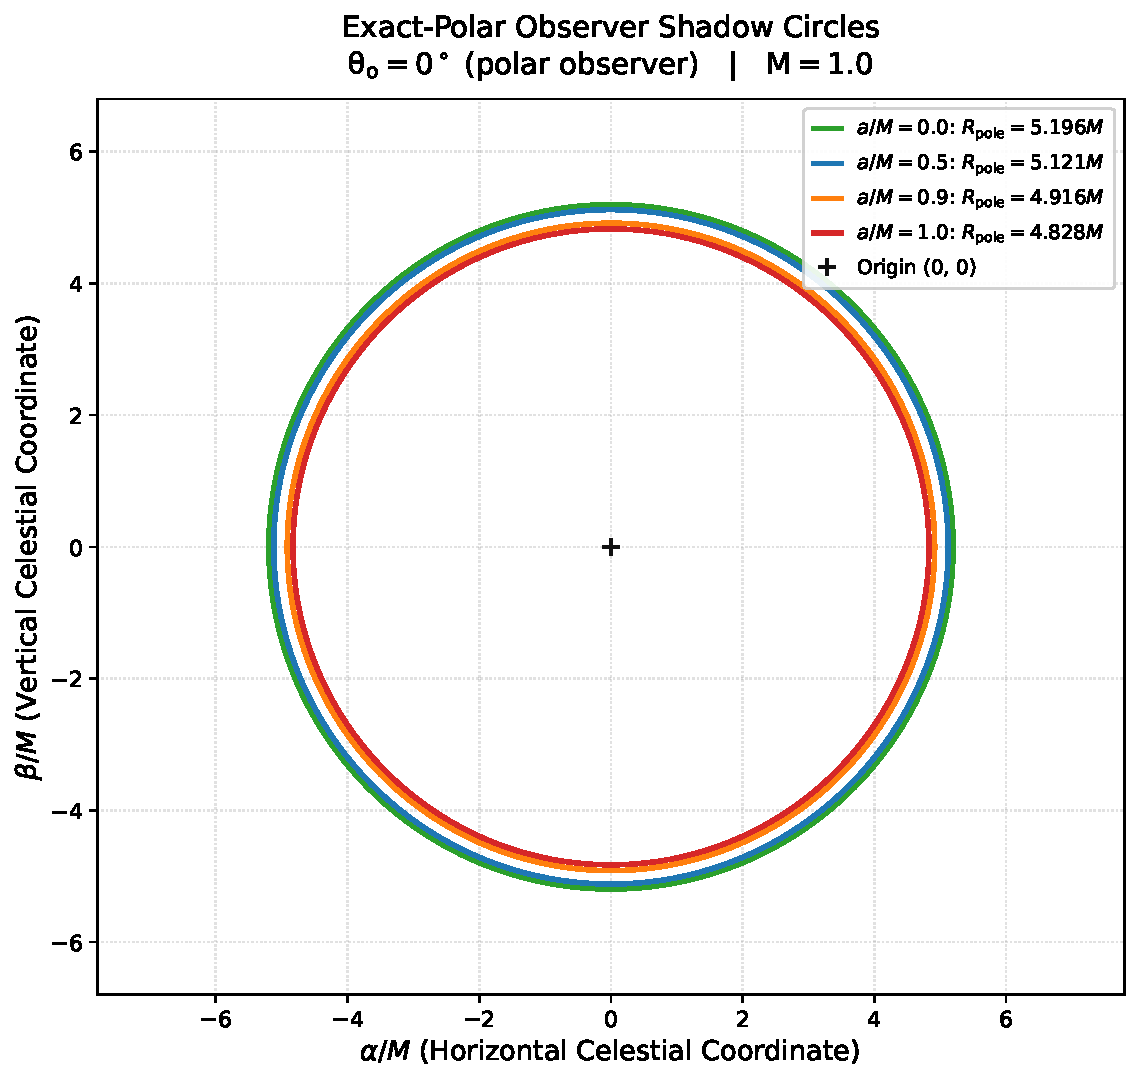
\includegraphics[width=0.58\textwidth]{exact_polar_shadow.pdf}
    \caption{Exact-polar observer shadow boundaries ($\theta_o = 0^\circ$) across black hole spins $a/M \in \{0.0, 0.5, 0.9, 1.0\}$. All boundaries are concentric circles centered at the origin, with radii contracting monotonically from $R_{\rm pole} = 3\sqrt{3}M \approx 5.196M$ ($a=0$) down to $R_{\rm pole} = 2(1+\sqrt{2})M \approx 4.828M$ ($a=M$).}
    \label{fig:exact_polar_shadow}
\end{figure}
